\documentclass[twocolumn,10pt,a4paper]{article}
\usepackage[french]{babel}
\usepackage[T1]{fontenc}
\usepackage[utf8]{inputenc} 
\usepackage{amsmath}
\usepackage{amsfonts}
\usepackage{amssymb}
\usepackage{graphicx}
\usepackage{verbatim}
\usepackage{listings}
\usepackage[usenames]{color}
\usepackage[left=1cm,right=1cm,top=2cm,bottom=2cm]{geometry}
\date{18 Septembre 2015}
\lstdefinestyle{customc}{
  belowcaptionskip=1\baselineskip,
  breaklines=true,
  frame=L,
  xleftmargin=\parindent,
  language=Matlab,
  showstringspaces=false,
  basicstyle=\footnotesize\ttfamily,
  keywordstyle=\bfseries\color{green},
  commentstyle=\itshape\color{black},
  identifierstyle=\color{blue},
  stringstyle=\color{blue},
%  backgroundcolor=\color{lightgray},
  extendedchars=true,
  showspaces=false,
  %numbers=left,
  %numberstyle=\footnotesize\ttfamily,
  %numbersep=9pt,
  %tabsize=2,
  breaklines=true,
  showtabs=false,
  %frame=leftline,
  caption=\lstname,
%  prebreak = \raisebox{0ex}[0ex][0ex]{\ensuremath{\hookleftarrow}}
  literate={\$}{{\textcolor{blue}{\$}}}1
}
\lstset{escapechar=@,style=customc}

\begin{document}
\title{\textbf{M2R ENEL - ENSE3 3A IEE} \\ BE1 : Algorithmes d'optimisation, non linéaire, déterministes, sans contraintes, mono-variable}
\author{\textit{Barnabé POTEL - Zakariya ZIANI}}
\maketitle


Le but de ce TP est de comprendre le fonctionnement des principales techniques d'optimisation basiques et de mettre en oeuvre des algorithmes simples.
\section{Stratégie manuelle}
\paragraph{Estimation du minimum de la fonction\\}
\begin{figure}[!h]
\centering
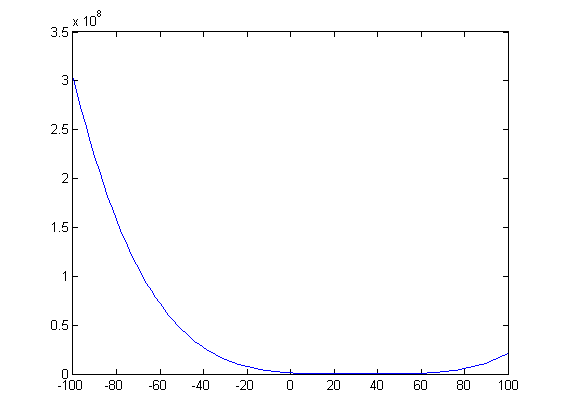
\includegraphics[width=6cm]{courbe1} 
\caption{Fonction sur l'intervalle [-100 100]}
\end{figure}
Premier intervalle : [0 60]\\
Deuxième intervalle : [20 40]\\
Troisième intervalle : [30 34]\\
....
On divise l'intervalle par environ 3 à chaque coup,

Il faut alors entre 11 et 12 itérations pour obtenir une solution sur l'intervalle précise de l'ordre de $10^{-4}$ :
$$\dfrac{200}{3^{11}}\sim 10^{-3} $$
$$\dfrac{200}{3^{12}}\sim 10^{-6} $$

\begin{figure}[!h]
\centering
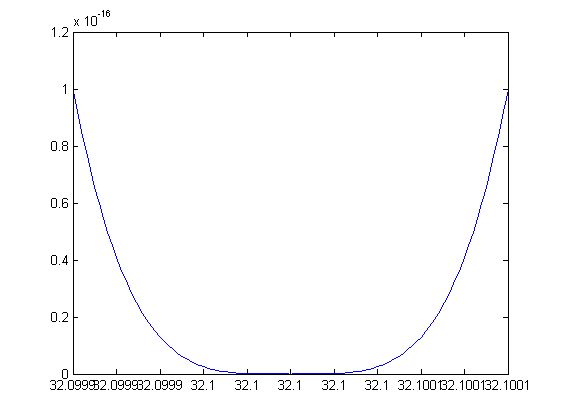
\includegraphics[width=6cm]{courbe2} 
\caption{Fonction sur l'intervalle [-100 100]}
\end{figure}

\section{Dichotomie}
Il est justifié d'utiliser la dichotomie car la fonction utilisée est convexe.

\paragraph{Execution de l'algorithme}
$X_{inf}= 32.1$\\
$X_{sup}=32.1001$\\
$iter=21$\\
$nbf=47$
\paragraph{Comparaison avec la stratégie manuelle}
La dichotomie est forcément plus rapide car automatisée (bien qu'une dichotomie manuelle soit possible aussi). Néanmoins le nombre d'itérations est plus important (21 au lieu d'environ 11) mais le nombre d'appel à la fonction est plus faible : 47 au lieu de 11*100=1100 fois par la stratégie manuelle.

\section{Section dorée}
\paragraph{Execution de l'algorithme}
$X_{inf}= 32.1$\\
$X_{sup}=32.1$\\
$iter=31$\\
$nbf=35$

\paragraph{Comparaison avec la stratégie manuelle}
Le nombre d'itération est supérieur à celui de la dichotomie mais ne nombre d'utilisation de la fonction est inférieure.

\section{Approximation parabolique}
Le principe de l'approximation parabolique est de considérer notre fonction comme un polynome du second degré dont on estime les coefficients par le calcul de sa valeur en trois points choisis. On peut connait alors le minimum de ce polynome qui représente notre fonction. On resserre ensuite l'intervale autour de ce minimum pour réévaluer plus finement notre fonction et converger vers son minimum réel.

\paragraph{Execution de l'algorithme}
$X_{inf}= 32.1$\\
$X_{sup}=32.1$\\
$iter=10$\\
$nbf=32$

\section{Algorithme hybride}
La fonction fminbnd de MATLAB calcul le minimum de la fonction en utilisant l'algorithme le plus adapté à chaque itération suivant les calculs réalisés précédemmment. Le nombre d'appels à la fonction peut alors varier à chaque itération.
\paragraph{Execution de l'algorithme}
\begin{lstlisting} 
 Func-count     x          f(x)      Procedure
    1       -23.6068  9.63014e+06     initial
    2        23.6068      5203.38     golden
    3        52.7864       183122     golden
    4        37.0873      618.691     parabolic
    5        30.7618      3.20723     parabolic
    6        33.1287      1.11994     parabolic
    7         31.963   0.00035205     parabolic
    8        32.2327  0.000310516     parabolic
    9         32.098  1.74643e-11     parabolic
   10        32.1021  1.98595e-11     parabolic
   11           32.1   1.2384e-18     parabolic
   12           32.1  1.22809e-18     parabolic
   13        32.0999  2.02732e-17     parabolic
 
Optimization terminated:
 the current x satisfies the termination criteria using OPTIONS.TolX of 1.000000e-04 

\end{lstlisting}
\section{Fonction plus complexe}
En recherchant un minimum sur l'intervalle [-10 10], l'algorithme converge vers un minimum local situé à -0.76 alors que le minimum global est situé à 6.69.

\begin{figure}[!h]
\centering
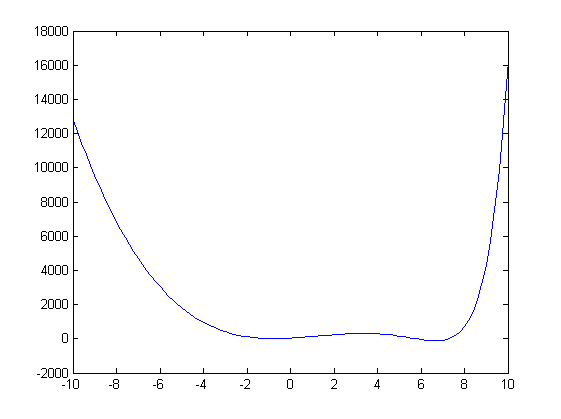
\includegraphics[width=6cm]{courbe3} 
\caption{Fonction plus complexe sur l'intervalle [-10 10]}
\end{figure}


\begin{lstlisting}
 Func-count     x          f(x)     Procedure
  1       -6.18034      3299.94    initial
  2       -3.81966       835.57    golden
  3       -2.36068      196.451    golden
  4       -1.70931      67.7314    parabolic
  5       -1.16778      17.2215    parabolic
  6      -0.905356      8.13884    parabolic
  7      -0.799407      6.96653    parabolic
  8      -0.765827      6.87575    parabolic
  9       -0.76006      6.87343    parabolic
 10      -0.759504      6.87341    parabolic
 11      -0.759471      6.87341    parabolic
 12      -0.759437      6.87341    parabolic
 
Optimization terminated:
 the current x satisfies the termination criteria using OPTIONS.TolX of 1.000000e-04 
x =

   -0.7595

\end{lstlisting}

On peut alors diviser l'intervalle initial de [-10 10] en deux intervalles : [-10 0] et [0 10] afin de trouver le minimum sur chaque intervalle :

\begin{lstlisting}
Func-count     x          f(x)         Procedure
 1        3.81966      301.327        initial
 2        6.18034     -73.0188        golden
 3        7.63932      232.408        golden
 4        5.82315     -7.10317        parabolic
 5         6.4272      -105.85        parabolic
 6        6.89019     -109.582        golden
 7        6.68159      -120.08        parabolic
 8        6.67625     -120.052        parabolic
 9        6.68903     -120.097        parabolic
10        6.69017     -120.097        parabolic
11        6.69013     -120.097        parabolic
12         6.6901     -120.097        parabolic
 
Optimization terminated:
 the current x satisfies the termination criteria using OPTIONS.TolX of 1.000000e-04 


x =

    6.6901
\end{lstlisting}
On a alors confirmation que $x=6.6901$ est bien le minimum global car la fonction en ce point vaut $\sim -120.1<f(0.759437)=6.87341$
\section{Méthode de Newton1D}
\paragraph{Convergence}
\subparagraph*{Point initial : -5}
Nombre d'itérations : 6
Nombre d'appel à la fonction : 7
X : -0.7595
\subparagraph*{Point initial : 0}
Nombre d'itérations : 4
Nombre d'appel à la fonction : 5
X : -0.7595
\subparagraph*{Point initial : 5}
Nombre d'itérations : 6
Nombre d'appel à la fonction : 7
X : 6.6901\\

Cette méthode permet de converger rapidement (par rapport aux précedents algorithmes) vers des minimas locaux. Il faut alors bien choisir le point initial pour tomber sur le minimum global. De par la rapidité de la méthode on peut alors la tester pour différents points initiaux répartis dans l'intervalle de travail et vérifier lequel correspond au minimul global en comparants les valeurs des fonctions en ces points.
\paragraph{Nous avons du rajouter une condition sur le Hessien afin de ne pas converger vers un maximum local pour le point initial 5}

\section*{Conclusion}
La dernière méthode utilisée : Newton1D permet une convergence bien plus rapide que l'ensemble des autres méthodes utilisées avant (notamment Dichotomie, Section Dorée et Approximation Parabolique). Tous ces algorithmes ne permettent pas forcément de trouver le minimum global. Il peut alors etre intéressant de "mailler" l'intervalle initial ou de prendre différents points initiaux dans cet intervalle pour comparer la convergence sur ces différentes portions.

\newpage
\newpage
\newpage
\section{ANNEXES}
\subsection{Section dorée}
\begin{lstlisting}
function [xinf,xsup,iter,nbf]=nombreor(fonc1D, xmin, xmax, maxiter, eps)

iter=0;         % initialisation du compteur d'iterations
nbf=0;          % initialisation du compteur d'appel a la fonction

x1=xmin;
x4=xmax;
x3=((x4-x1)*2)/(1+sqrt(5))+x1;
x2=x4+x1-x3;
%calcul les 4 valeurs de f en x1, x2, x3, x4
f1=feval(fonc1D,x1);
f2=feval(fonc1D,x2);
f3=feval(fonc1D,x3);
f4=feval(fonc1D,x4);
nbf=nbf+4;

while(iter<maxiter && (x4-x1)>eps)
    iter=iter+1;
    
    if (f1<f2 & f2<f3 & f3<f4) % On doit recalculer x2 et x3
        y1=x1;          z1=f1;
        y4=x2;          z4=f2;
        y3=((y4-y1)*2)/(1+sqrt(5))+y1;      z3=feval(fonc1D,y3);
        y2=y4+y1-y3;    z2=feval(fonc1D,y2);    nbf=nbf+2;
    elseif (f1>f2 & f2<f3 & f3<f4)  % On doit recalculer x2
        y1=x1;          z1=f1;
        y3=x2;          z3=f2;
        y4=x3;          z4=f3;
        y2=y4+y1-y3;    z2=feval(fonc1D,y2);    nbf=nbf+1;
    elseif (f1>f2 & f2>f3 & f3<f4)  % On doit recalculer x3
        y1=x2;          z1=f2;
        y2=x3;          z2=f3;
        y4=x4;          z4=f4;
        y3=y4+y1-y2;    z3=feval(fonc1D,y3);    nbf=nbf+1;
    elseif (f1>f2 & f2>f3 & f3>f4)  % On doit recalculer x2 et x3
        y1=x3;          z1=f3;
        y4=x4;          z4=f4;
        y3=((y4-y1)*2)/(1+sqrt(5))+y1;      z3=feval(fonc1D,y3);
        y2=y4+y1-y3;    z2=feval(fonc1D,y2);    nbf=nbf+2;
   else
        disp('fonction probablement non convexe ou constante');
        
    end
    x1=y1;      f1=z1;
    x2=y2;      f2=z2;
    x3=y3;      f3=z3;
    x4=y4;      f4=z4;
end

xinf=x1;
xsup=x4;
\end{lstlisting}
\newpage
\subsection{Parabolique}
\begin{lstlisting} 
function [xinf,xsup,iter,nbf] = para( fonc1D, xmin, xmax, maxiter, eps )
iter=0; %initialisation du compteur d'iterations
nbf=0;  %initialisation du compteur d'appel a la fonction

x1=xmin;
x3=xmax;

f1=feval(fonc1D,x1);
f3=feval(fonc1D,x3);
nbf=nbf+2;


while(iter<maxiter && (x3-x1)>eps)
    iter=iter+1;
    x2=(x1+x3)/2; % On choisit le troisieme point comme le milieu de l'intervalle choisi
    f2=feval(fonc1D,x2);
    xopt=(x1^2*(f2-f3)+x2^2*(f3-f1)+x3^2*(f1-f2))/(2*(x1*(f2-f3)+x2*(f3-f1)+x3*(f1-f2)));
    interval=x3-x1;
    x1=xopt-interval/10;      f1=feval(fonc1D,x1); % On reprend un intervalle 5 fois plus petit que precedemment
    x3=xopt+interval/10;      f3=feval(fonc1D,x3);
    nbf=nbf+3;
end

xinf=x1;
xsup=x3;
\end{lstlisting} 
\newpage
\subsection{Newton 1D}
\begin{lstlisting} 
function [x, fn, iter, fncall] = newton1D(fonc1D, xini, maxiter, eps)

iter=0;         % initialisation du compteur d'iterations
fncall=0;          % initialisation du compteur d'appel a la fonction

x1=xini;

%calcul des derivees de la fonction
[f, fp, fs]=fonction1D(x1);
fncall=fncall+1;
d=1;

while(iter<maxiter && d>eps)
    iter=iter+1;
    if fs<0 % Cette condition permet de ne pas se faire pieger par un maximum
        y1=x1+fp/fs;
    else
        y1=x1-fp/fs;
    end
    [f, fp, fs]=fonction1D(y1);
    fncall=fncall+1;
    d=abs(x1-y1); % Une condition d'arret est l'evolution entre deux points estimes
    x1=y1
end
x=x1;
fn=f;
fs
end

\end{lstlisting} 


\end{document}